\section{Wstep teoretyczny} \label{theory}
W kolejnych podrozdziałach opisane są krótko podstawy teoretyczne dotyczące uczenia maszynowego, wykorzystanych algorytmów oraz użytych metod optymalizacji.
\subsection{Formalny opis uczenia maszynowego}
Formalną definicję uczenia maszynowego podał Tom Mitchell, która brzmi następująco: ,,Mówimy, że maszyna uczy się zadania $T$ w oparciu o doświadczenie $E$ i miarę jakości $P$, jeśli wraz z przyrostem doświadczenia $E$ poprawia się jakość wykonywanego zadania $T$ mierzona przez miarę $P$.''\cite{mitchel} Przykładowo można wymienić trójkę $T$, $E$, $P$ jako diagnozowanie pacjenta na podstawie symptomów, dotychczasowe  liczba wykonanych przez maszynę diagnoz (poprawnie lub nie),  poprawność diagnozowania na podstawie do tej pory niespotkanych przypadków. Powyższe przykłady można mnożyć. Zapis formalny (na podstawie \cite{formal2}) w przypadku algorytmów przedstawionych w nieniejszej pracy możemy przedstawić następująco:
\begin{itemize}
\item $x$ - dane wejściowe algorytmu
\item $y$ - wyjście algorytmu
\item $f$ - funkcja modelowana
\item $g$ - funkcja modelująca.
\end{itemize}
Ogólnie możemy powiedzieć, że zadaniem algorytmu jest znalezienie takiej funkcji $g$, która jak w najlepszy stopniu przybliża funkcję $f$. Odnosząc to do przykładu rozpoznawania chorób, możemy powiedzieć, że modelowaną funkcją jest funkcja symptomów, która przyporządkowuje pacjentowi diagnozę. Uczenie wg danego algorytmu przeprowadza się na podstawie danych:
\begin{equation}
d = (x_1,y_1), (x_2, y_2), ..., (x_n, y_n).
\end{equation}
Każda para $(x_i, y_i)$ stanowi jeden rekord danych lub też jeden przykład podawany do algorytmu. W odniesieniu do przykładu z rozpoznawaniem chorób na podstawie symptomów, jednym rekordem jest konkretny zestaw symptomów ($x_i$) wraz z diagnozą ($y$).  Ogólniej, poszczególne symptomy nazywa się cechami lub atrybutami. W zależności od tego czy $y$ przyjmuje wartości ciągłe czy dyskretne, mamy do czynienia z wykorzystaniem uczenia maszynowego w problemie kolejno regresji lub klasyfikacji. 
%W tej pracy wszystkie metody optymalizacji były analizowane pod kątem problemu klasyfikacji lecz naturalne jest ich użycie w przypadku problemu regresji.

\subsection{Wykorzystane algorytmy}
W tym podrozdziale opisane są kolejne algorytmy, które wykorzystywane były w pracy.
\subsubsection{Drzewo decyzyjne}
%www.cs.princeton.edu/courses/archive/spr07/cos424/papers/mitchell-dectrees.pdf
% scikit-learn uses an optimised version of the CART algorithm.
Drzewo decyzyjne jest algorytmem uczenia maszynowego, który może posłużyć w celu rozwiązania problemu klasyfikacji oraz regresji. Funkcja, która jest modelowana przez algorytm przedstawiana jest w formie drzewa matematycznego. Jest to jedna z najpopularniejszych metod, która znalazła swoje wykorzystanie w diagnozowaniu chorób czy ocenie ryzyka kredytowego klientów banków\cite{mitchel}. Zaletami tego podejścia jest między innymi  prostota oraz łatwość interpretacji. Dużą wadą drzew decyzyjnych jest fakt, iż stworzenia optymalnego drzewa decyzyjnego należy do klasy problemów NP-zupełnych. W praktyce tworzenie drzewa oparte jest na metodach heurystycznych\cite{dtscikit}. Na rysunku \ref{dt1image} przedstawione zostało przykładowe drzewo, które mogłoby posłuży do klasyfikacji danych o trzech atrybutach na trzy klasy. Można stwierdzić, że drzewo decyzyjne jest tzw. białą skrzynką (\textit{whitebox}), ponieważ łatwo można zauważyć na jakiej podstawie podjęta została decyzja przyporządkowania do danej klasy.

\begin{figure}[ht!]
\centering
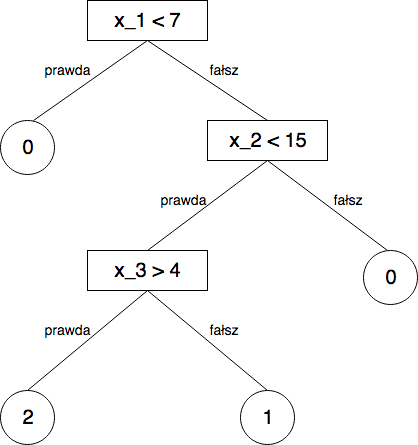
\includegraphics[scale=0.4]{res/dt1.png}
\caption[Caption for LOF]{Przykład drzewa decyzyjnego\label{dt1image}}
% \caption{Matematyczny model neuronu\label{neuron} Źródło:\footnote{aa} } 
\end{figure} 

\paragraph{Tworzenie drzewa decyzyjnego}\mbox{}\\
%ftp://ftp.boulder.ibm.com/software/analytics/spss/support/Stats/Docs/Statistics/Algorithms/14.0/TREE-CART.pdf
Istnieją różne sposoby na stworzenie drzewa klasyfikacyjnego. Jednym z nich jest algorytm CART -\textit{Classification  and  Regression  Trees}, który był wykorzystany w tej pracy i jest opisany w tym paragrafie. Ideą tego podejścia jest dzielenie danych wejściowych na rozłączne i dopełniające się podzbiory w taki sposób, aby zbiory te pozostawały jak najbardziej jednorodne tj. posiadały jak najwięcej rekordów przynależących do tej samej kategorii. Budowa drzewa zaczyna się od jego korzenia. Wybieramy atrybut wg którego chcemy podzielić dane na dwa jak najbardziej jednorodne zbiory. Po podzieleniu zbioru na dwa podzbioru postępujemy tak samo z następnymi atrybutami. Podział przeprowadzany jest aż do momentu, gdy wszystkie rekordy w każdym podzbiorze przynależą do tej samej kategorii. Należy jednak określić wg których atrybutów dzielić dane tak aby powstawały jak najbardziej jednorodne zbiory. W tym celu wykorzystywane są różnego rodzaju kryteria jednorodności\cite{CART}. Cały algorytm, w uproszczeniu, można opisać w dwóch krokach:
\begin{enumerate}
\item Wybór atrybutu, który pozwoli podzielić zbiór na dwa najbardziej jednorodne podzbiory.
\item Podział wg atrybutu wybranego w kroku 1 jeżeli nie zostały spełnione warunki końca algorytmu\cite{CART}.
\end{enumerate}
Warunkiem końca algorytmu może być sytuacja w której wszystkie stworzone podzbiory są jednorodne lub też moment, gdy dotarliśmy do maksymalnej głębokości drzewa. Każdy podzbiór oznacza kolejną gałąź w drzewie, co powoduje wzrost drzewa. Gdy drzewo jest zbyt duże, staję się ono zbyt skomplikowane i podatne na przeuczenie(\textit{overfitting}). Jednym z parametrów drzewa decyzyjnego, który należy określić jest właśnie jego maksymalna głębokość, która pozwala stworzyć optymalne drzewo. Wspomniany problem przeuczenia został opisany w podrozdziale \ref{problems}. 

\subsubsection{Las drzew decyzyjnych}
\subsubsection{Maszyna wektorow nosnych}
\subsubsection{Tradycyjne sieci neuronowe}
\subsubsection{Glebokie sieci neuronowe}
\subsection{Wykorzystane metody optymalizacji}
\subsubsection{Walidacja krzyzowa - wyznaczanie parametrow modelu}
\subsubsection{Sztuczne powiekszanie zbioru danych}
\subsubsection{Ekstrakcja cech}
\subsection{Problemy wynikające z niskiej ilości danych?}\label{problems}
\subsection{Proponowane rozwiązania?}
\paragraph{LDA}
\paragraph{PCA}

